\documentclass[10pt,a4paper]{report}
\usepackage[latin1]{inputenc}
\usepackage{amsmath}
\usepackage{amsfonts}
\usepackage{amssymb}
\usepackage{graphicx}
\usepackage{hyperref}
\usepackage{multicol}
\usepackage[margin=0.5in]{geometry}
\usepackage{tikz}
\usepackage{romannum}
\usepackage{listings}
\usetikzlibrary{arrows,shapes.gates.logic.US,shapes.gates.logic.IEC,calc}
\usepackage{titlesec}
\titlespacing{\subsection}{1pt}{\parskip}{3pt}
\titlespacing{\subsubsection}{0pt}{\parskip}{-\parskip}
\titlespacing{\paragraph}{0pt}{\parskip}{\parskip}
\newcommand{\myvec}[1]{\ensuremath{\begin{pmatrix}#1\end{pmatrix}}}
\let\vec\mathbf

\begin{document}

\centering {
\includegraphics[scale=0.07]{IIT.png}} \vspace{3mm}\\ \raggedleft Name:Somisetty.Kedareswari\vspace{2mm}\\ \raggedleft Roll No.: FWC22049\vspace{2mm}\\ \raggedright Sep 2022 \hspace{12cm} \raggedleft mail2kedari@gmail.com \vspace{10mm}
\\ \centering \Large \textbf{MATRIX ASSIGNMENT} \normalsize \vspace{15mm}
\begin{multicols}{2}
\section{Problem:}  Let C be the circle with centre (0, 0) and radius 3 units. To find the equation of the locus of the mid points of the chords of the circle C that subtend an angle of 2$\pi$/3 at its \raggedright center\vspace{3mm}
\section{Solution}
The input parameters for this construction are
\begin{center}
\begin{tabular}{|c|c|c|}
  \hline
  \textbf{Symbol}&\textbf{Value}&\textbf{Description}\\
  \hline
  r & 3cm & Radius of a circle given as 8cm\\
  \hline
  $\angle{AOB}$ & $120^0$ & Angle between two chords\\
  \hline 
  O & $\myvec{0\\0}$ & Centre Point\\
  \hline
  A & $\myvec{rcos \theta \\ rsin \theta }$ &  Point A from Origin\\
  \hline
  B & $\myvec{ rcos\theta \\ -rsin\theta}$ & Point B from Origin\\
  \hline
\end{tabular}
\end{center}
\raggedright\textbf{Caluclating Locus:} \\
\raggedright The two chords of a circle A and B substend at an angle 2$\pi$ /3 at its Centre are $\myvec{1.5 \\ 2.5}$ and $\myvec{ 1.5 \\ -2.5}$ respectively.\\(Using formulae to finding a point on circle from origin)\\
  \centering Finging mid-point of the line joining the chords is \\ 
   \centering    \begin{equation} M=(A+B)/2. \end{equation} \\
  We have the Centre point and the mid point of the chords of the circle,so we can find radius and can form the locus(circle) which is joining all the possible chords.
 \\ For Finding Radius(r2) \\ Direction Vector of the two  points will be \\     \begin{equation} 
  r2 \implies (O-M)=\sqrt{M.M^T} 
 \end{equation}\\ 
 
   Circle Equation is \\
   \begin{equation} 
     (x-x0)^2+(y-y0)^2=r2^2
   \end{equation}\\ 
   \begin{equation} 
   Where, (x0,y0)=\myvec{0\\0} 
  \end{equation} \\
  so,by caluclating we get
   $x^2+y^2= r2^2$ \\
   Equation of locus is
   \begin{equation}
    x^2+y^2= 2.25
   \end{equation}
   
 \begin{center}
Below python code realizes the above construction : 
\fbox{\parbox{8.5cm}{\url{https://github.com/kedareswari200/fwc-moudle1/blob/Matrix_Circle/cir.py}}}
\end{center}
 \section{Construction}
   \begin{center}
  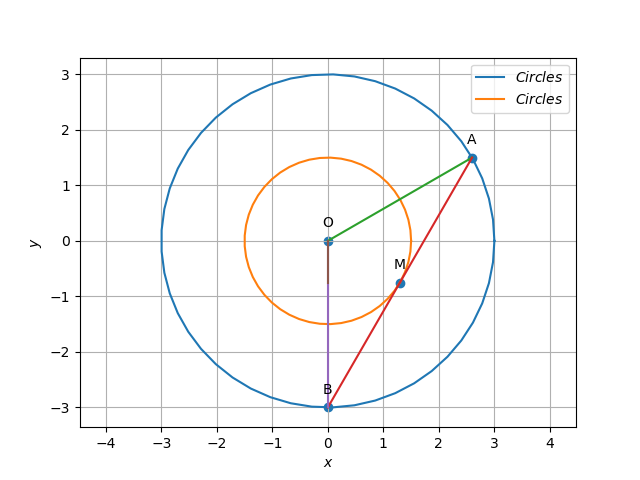
\includegraphics[scale=0.5]{Fig.png}
    \end{center}
\vspace{3cm}
\end{multicols}

\end{document}